% !TeX spellcheck = nl
\documentclass[]{subfiles}
\begin{document}
	\section{Convolutie stelling}
	Toepassen van de definitie van Laplace transformatie.
	\begin{equation}
		\Lapl\left[ f(t)\ast g(t)\right]  = \int_{0}^{+\infty}\left[ f(t)\ast g(t)\right] e^{-st}dt
	\end{equation}
	Toepassen van de definitie van de convolutie
	\begin{equation}
		\int_{0}^{+\infty}\left[ \int_{-\infty}^{+\infty}f(\tau)g(t-\tau)d\tau	\right] e^{-st}dt
	\end{equation}
	Toepassen van de causale eigenschap
	\begin{equation}
		\int_{-\infty}^{+\infty}\left[ \int_{0}^{t}f(\tau)g(t-\tau)d\tau\right] e^{-st}dt
	\end{equation}
	Wisselen van de integralen
	\begin{equation}
		\int_{0}^{+\infty}f(\tau)\left[ \int_{\tau}^{+\infty}g(t-\tau)e^{-st}dt\right] d\tau
	\end{equation}
	Tekeningske om uit te leggen hoe de grenzen werken:
	\begin{figure}[h]
		\centering
		\begin{subfigure}{.4\textwidth}
			\begin{center}
				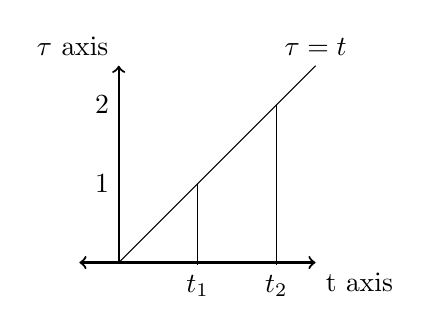
\begin{tikzpicture}
					\centering
					\draw[thick,<->] (-0.5,0) -- (2.5,0) node[anchor=north west] {t axis};
					\draw[thick,->] (0,0) -- (0,2.5) node[anchor=south east] {$\tau$ axis};
					\foreach \x in {1,2}
					\draw (\x cm,1pt) -- (\x cm,-1pt) node[anchor=north] {$t_{\x}$};
					\foreach \y in {1,2}
					\draw (0,\y cm) -- (0,\y cm) node[anchor=east] {$\y$};
					\draw[black] (0,0) -- (2.5,2.5) node[anchor=south] {$\tau = t$} ;
					\draw[black] (1,0) -- (1,1) ;
					\draw[black] (2,0) -- (2,2) ;
					%TODO:  zorg dat de opp onder de lijn gekleurd is 
				\end{tikzpicture}
			\end{center}
			\caption{Voor}
		\end{subfigure}%
		\begin{subfigure}{.4\textwidth}
			\begin{center}
				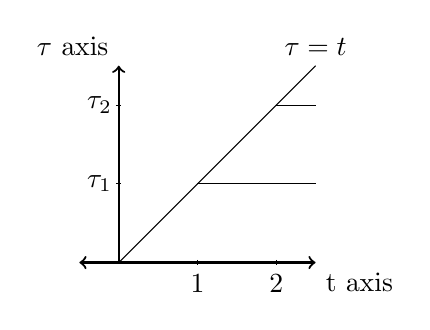
\begin{tikzpicture}
						\centering
						\draw[thick,<->] (-0.5,0) -- (2.5,0) node[anchor=north west] {t axis};
						\draw[thick,->] (0,0) -- (0,2.5) node[anchor=south east] {$\tau$ axis};
						\foreach \x in {1,2}
						\draw (\x cm,1pt) -- (\x cm,-1pt) node[anchor=north] {$\x$};
						\foreach \y in {1,2}
						\draw (-1pt,\y cm) -- (+1pt,\y cm) node[anchor=east] {$\tau_{\y}$};
						\draw[black] (0,0) -- (2.5,2.5) node[anchor=south] {$\tau = t$} ;
						\draw[black] (1,1) -- (2.5,1) ;
						\draw[black] (2,2) -- (2.5,2) ;
						%TODO:  zorg dat de opp onder de lijn gekleurd is 
				\end{tikzpicture}
			\end{center}
			\caption{Na}
		\end{subfigure}
		\caption{Te convolueren pulsen}
		\label{fig:grenzenLaplace}
	\end{figure}
	\begin{equation}
		\left\{ \begin{array}{r@{\text{ $\rightarrow$ }}l}
			\tau:0&t \\
			 t:0&+\infty 
		\end{array}\right.\quad\Rightarrow\quad
	\left\{ \begin{array}{r@{\text{ $\rightarrow$ }}l}
		\tau:0&+\infty\\
		t:\tau&+\infty 
	\end{array}\right.
	\end{equation}
	We passen nu eigenschappen van de EXP toe:
	\begin{equation}
		\int_{0}^{+\infty}f(\tau)\left[ \int_{\tau}^{+\infty}g(t-\tau)\underbrace{e^{-s(t-\tau)}e^{-s\tau}}_{e^{-st}}dt\right]d\tau 
	\end{equation}
	We passen nu de lineariteit van de integraal toe:
	\begin{equation}
		\int_{0}^{+\infty}f(\tau)e^{-st}\left[ \int_{\tau}^{+\infty}g(t-\tau)e^{-s(t-\tau)}dt\right] d\tau
	\end{equation}
	We passen nu een substitutie toe: $u = t-\tau  \Rightarrow du = dt \Rightarrow u: 0\rightarrow+\infty$
	\begin{equation}
		\int_{0}^{+\infty}f(\tau)e^{-st}\left[ \underbrace{\int_{0}^{+\infty}g(u)e^{-su}du}_{=G(s)}\right] d\tau
	\end{equation}
	We passen nu de lineariteit van de integraal toe:
	\begin{equation}
		G(s)\underbrace{\int_{0}^{+\infty}f(\tau)e^{-s\tau}d\tau}_{=F(s)}=G(s)F(s)
	\end{equation}
\end{document}